\documentclass[conference]{IEEEtran}
\usepackage[utf8]{inputenc}
\usepackage[spanish]{babel}
\usepackage{amsmath,amssymb,amsfonts}
\usepackage{graphicx}
\usepackage{cite}
\usepackage{hyperref}
\usepackage{float}
\usepackage{array}
\usepackage{booktabs}

\begin{document}

\title{Segmentación de Imágenes Médicas con Arquitectura U-Net}

\author{\IEEEauthorblockN{Juan Felipe Pardo Carrillo}
\IEEEauthorblockA{\textit{Dpto. de Ciencias de la Computación e Inteligencia Artificial} \\
\textit{Universidad de Sevilla}\\
Sevilla, España \\
juaparpar@alum.us.es (HHX3170)}
\and
\IEEEauthorblockN{Diego Vicente Cámara}
\IEEEauthorblockA{\textit{Dpto. de Ciencias de la Computación e Inteligencia Artificial} \\
\textit{Universidad de Sevilla}\\
Sevilla, España \\
dieviccam@alum.us.es (RXW1249)}
}

\maketitle

\begin{abstract}
El objetivo principal de este trabajo es construir, entrenar y evaluar una red neuronal convolucional basada en la arquitectura U-Net para segmentar automáticamente los vasos sanguíneos en imágenes del fondo de ojo pertenecientes al dataset público DRIVE 2004. Dada la gran complejidad típica de las imágenes oftalmológicas (presencia de ruido de adquisición, iluminación irregular y un contraste extremadamente bajo en los capilares finos) y la inherente escasez de muestras médicas etiquetadas, se ha diseñado un exhaustivo pipeline de preprocesamiento, aumento de datos y extracción de mosaicos espaciales (\textit{patching}). El preprocesamiento estandariza la señal visual a través de técnicas como la conversión a escala de grises y la normalización matemática de las intensidades de los píxeles. A nivel arquitectónico, la red U-Net se ha adaptado y regularizado mediante el uso de capas de Dropout y Batch Normalization para prevenir de forma activa el sobreajuste. Empleando una función de coste combinada y equilibrada (0.5 * BCE + 0.5 * Dice Loss), el modelo logra una segmentación robusta y precisa de las estructuras capilares. Este sistema sienta las bases para superar holgadamente los umbrales de rendimiento exigidos (DICE score $> 0.75$) frente a validaciones manuales de expertos clínicos, contribuyendo de forma significativa a la automatización del diagnóstico en patologías oculares y cardiovasculares como la retinopatía diabética.
\end{abstract}

\begin{IEEEkeywords}
Segmentación de Imágenes Médicas, Aprendizaje Profundo, Redes Neuronales Convolucionales, U-Net, DRIVE 2004, Preprocesamiento, Retinopatía Diabética, Patching, Inferencia, Skip Connections.
\end{IEEEkeywords}

\section{Introducción}
La visión artificial y el análisis automatizado de imágenes médicas han avanzado de manera disruptiva durante la última década gracias a la irrupción del Aprendizaje Profundo (\textit{Deep Learning}). La segmentación de imágenes biomédicas, entendida como el complejo proceso de partición digital de una imagen en segmentos semánticamente significativos a nivel de píxel, representa uno de los desafíos más críticos e investigados en la intersección actual entre la informática y la medicina moderna \cite{ref1, ref3}.

\subsection{La Relevancia Clínica de la Segmentación}
El análisis minucioso de la vasculatura retiniana a través de imágenes del fondo de ojo constituye un procedimiento clínico fundamental para el diagnóstico, monitorización y seguimiento de múltiples patologías cardiovasculares y oftalmológicas. Enfermedades de carácter silencioso pero con consecuencias severas, como la retinopatía diabética, la hipertensión arterial crónica o el glaucoma, dejan su primera huella clínica detectable en los diminutos capilares de la retina. Tradicionalmente, la delimitación y el seguimiento de esta intrincada red capilar ha sido realizada de manera puramente manual por oftalmólogos y especialistas. 

Sin embargo, este enfoque tradicional presenta graves limitaciones logísticas. Requiere un tiempo considerable de análisis por cada paciente, está fuertemente sujeto a la variabilidad intra e inter-observador (la alta subjetividad humana a la hora de delimitar qué constituye un vaso capilar muy fino y qué es simplemente ruido óptico) y dificulta enormemente la escalabilidad ante el volumen masivo de datos clínicos que se genera diariamente en los sistemas de salud. La automatización de este proceso mediante herramientas de Inteligencia Artificial promete ofrecer una segunda opinión diagnóstica que sea instantánea, constante, repetible y completamente libre de la fatiga visual humana.

\subsection{Desafíos Computacionales}
La automatización algorítmica de este proceso clínico enfrenta notables obstáculos técnicos inherentes a la propia naturaleza de la fotografía médica. Las imágenes del fondo de ojo se adquieren dilatando la pupila del paciente y proyectando un fuerte haz de luz hacia el interior del globo ocular. Esta técnica provoca deslumbramientos y reflejos inevitables sobre la lente y la propia retina. Entre los retos computacionales más destacados a los que debe sobreponerse el algoritmo se encuentran: la alta variabilidad en la iluminación entre diferentes capturas, el ruido térmico de los sensores fotográficos, el reducidísimo contraste existente entre los vasos capilares más distales y el tejido retiniano de fondo, y la posible presencia de anomalías patológicas (como hemorragias o exudados lipídicos) que el sistema informático es susceptible de confundir con estructuras vasculares \cite{ref4}.

\subsection{Solución Propuesta}
En respuesta a estas severas limitaciones fotográficas y analíticas, las arquitecturas de Redes Neuronales Completamente Convolucionales (\textit{Fully Convolutional Networks}, FCN) se han consolidado como el estándar de la industria en el análisis de imagen médica. En particular, la arquitectura U-Net, propuesta por Ronneberger et al. \cite{ref3}, destaca profundamente en la literatura científica por su eficacia. Su diseño inteligente combina una ruta de contracción progresiva para capturar el contexto global de la imagen (saber qué elementos hay) y una ruta de expansión simétrica para recuperar la precisión espacial original (saber exactamente dónde están ubicados) mediante el uso de conexiones de salto (\textit{skip connections}). Esta topología permite entrenar modelos extremadamente robustos partiendo de un conjunto muy reducido de imágenes anotadas, una ventaja logística crucial en el ámbito médico donde la obtención de datos etiquetados por expertos es sumamente costosa. El presente trabajo detalla paso a paso el diseño algorítmico, las decisiones de arquitectura de red y la justificación matemática de las métricas empleadas para abordar este problema de segmentación.

\section{Dataset y Objetivo}
El conjunto de datos utilizado de manera exclusiva para el entrenamiento, la validación y el testeo del modelo es el reconocido repositorio DRIVE (\textit{Digital Retinal Images for Vessel Extraction}) \cite{ref7}. Publicado originariamente en el año 2004, su rigor clínico lo mantiene hoy en día como un estándar global ineludible para evaluar y comparar algoritmos de extracción vascular.

\begin{figure}[htbp]
    \centering
    \includegraphics[width=\linewidth]{demo_01_raw_samples.png}
    \caption{Muestras representativas del conjunto de datos DRIVE 2004. Se ilustra una imagen original RGB del fondo de ojo capturada mediante retinografía junto a su máscara de segmentación experta (\textit{Ground Truth}), donde los píxeles blancos indican la red vascular confirmada. Se observa claramente la complejidad topológica, el ruido lumínico y el bajo contraste en las ramificaciones distales.}
    \label{fig:raw_samples}
\end{figure}

Como se detalla visualmente en la Fig. \ref{fig:raw_samples}, las imágenes base son fotografías a color RGB del fondo ocular. Dada la dificultad de su obtención, el dataset consta de únicamente 40 imágenes originales, cada una con una resolución nativa de $565 \times 584$ píxeles. Estas fotografías fueron obtenidas durante un programa real de detección temprana masiva de retinopatía diabética llevado a cabo en los Países Bajos. Del total de la cohorte clínica, siete de las capturas presentan signos incipientes de la patología, mientras que las 33 fotografías restantes corresponden a pacientes sanos, dotando al modelo de ejemplos tanto normativos como patológicos.

\subsection{División de los Datos Clínicos}
La distribución de los datos se estructura metodológicamente en dos conjuntos estrictamente separados para asegurar una evaluación rigurosa y evitar que el modelo memorice la casuística:
\begin{itemize}
    \item \textbf{Conjunto de Entrenamiento (\textit{Training Set}):} Contiene 20 imágenes equipadas con sus máscaras del campo de visión útil (FOV) y una máscara de segmentación binaria perfecta etiquetada manualmente por un oftalmólogo experto. Para maximizar la capacidad de generalización durante la fase de aprendizaje, la validación interna del algoritmo se gestiona dinámicamente mediante una estrategia de Validación Cruzada en 5 pliegues (\textit{5-Fold Cross-Validation}). Este método rota el particionado utilizando iterativamente un 80\% de las muestras para el ajuste de pesos y el 20\% restante para validación cruzada.
    \item \textbf{Conjunto de Prueba (\textit{Test Set}):} Incluye las 20 imágenes restantes no vistas por el modelo. A diferencia del conjunto de entrenamiento, esta partición dispone de segmentaciones realizadas por dos expertos clínicos independientes. Este factor es fundamental para la investigación, ya que permite evaluar el rendimiento del algoritmo comparándolo directamente contra la variabilidad inter-observador intrínseca al criterio humano.
\end{itemize}

\begin{table}[htbp]
\centering
\caption{Resumen del Pipeline de Datos y Experimentación}
\label{tab:pipeline_summary}
\begin{tabular}{@{}p{3.5cm}p{4.5cm}@{}}
\toprule
\textbf{Parámetro} & \textbf{Valor / Configuración} \\
\midrule
Total Muestras Crudas & 40 imágenes (DRIVE 2004) \\
Conjunto de Entrenamiento & 20 imágenes \\
Conjunto de Prueba (Test) & 20 imágenes \\
Mecanismo de Validación & 5-Fold Cross-Validation (Dinámico) \\
Resolución Original & $565 \times 584$ píxeles \\
Tamaño de Parche (\textit{Patch}) & $128 \times 128$ píxeles \\
Extracción (Entrenamiento) & Aleatoria (\textit{Random Cropping} dinámico) \\
Extracción (Inferencia) & Ventana deslizante (\textit{Stride} = 64) \\
Aumentos de Datos (\textit{Augmentation}) & Giros ortogonales y transposiciones especulares \\
\bottomrule
\end{tabular}
\end{table}

\textbf{Objetivo Principal del Trabajo:} El propósito central es implementar de manera integral, entrenar y evaluar rigurosamente una arquitectura convolucional U-Net que sea capaz de segmentar de forma automática los capilares sanguíneos en imágenes no vistas. El flujo de preprocesamiento extrae dinámicamente cientos de parches independientes por iteración (época). El reto analítico primario reside en que el modelo debe sobreponerse al fuerte desequilibrio de clases natural del dominio (las estructuras vasculares ocupan apenas entre un 10\% y un 15\% del campo de visión). Bajo estas condiciones adversas, el sistema debe superar una métrica media de DICE de \textbf{0.75} sobre el conjunto de test, debiendo calcularse este promedio contrastando las predicciones contra las máscaras de los \textbf{dos expertos clínicos} de forma independiente.

\section{Métricas de Evaluación}
La evaluación de la precisión predictiva en problemas de segmentación biomédica requiere el empleo de métricas estrictamente específicas, distanciándose de las métricas clásicas de clasificación general. Debido al severo desequilibrio de clases previamente mencionado, utilizar únicamente la Precisión Global (\textit{Accuracy}) resultaría una métrica inútil y altamente engañosa. Un modelo trivial o «perezoso» que simplemente se dedicara a clasificar la totalidad de los píxeles de cualquier imagen como tejido sano de fondo (la clase mayoritaria), superaría fácilmente una tasa de acierto del 85\% sin haber logrado detectar una sola estructura vascular.

Por este motivo, la evaluación computacional se apoya en métricas de superposición espacial. En nuestra implementación informática (\texttt{metrics.py}), se ha introducido de forma transversal un factor infinitesimal de suavizado ($\epsilon = 10^{-7}$). Esta adición garantiza la estabilidad numérica del entorno impidiendo excepciones por división por cero en aquellos recortes de imagen donde no existe ningún vaso sanguíneo presente.

\textbf{1) Coeficiente de Sørensen-Dice (DICE Score):} Constituye la métrica de rendimiento indiscutible en la literatura de segmentación médica. Evalúa matemáticamente el nivel de solapamiento o coincidencia exacta entre el mapa predictivo y el experto humano, penalizando agresivamente los errores y omitiendo por completo los Verdaderos Negativos (el amplio tejido de fondo irrelevante). Su rango abarca desde 0 (sin coincidencias) hasta 1 (superposición perfecta):
\begin{equation}
DICE = \frac{2 |X \cap Y| + \epsilon}{|X| + |Y| + \epsilon} = \frac{2 \cdot TP}{2 \cdot TP + FP + FN}
\end{equation}
donde $TP$ denota los Verdaderos Positivos, $FP$ los Falsos Positivos y $FN$ los Falsos Negativos. A nivel de ingeniería, se ha implementado mediante la clase especializada \texttt{DiceCoefficient} (heredando de \texttt{keras.metrics.Metric}) diseñada para acumular el estado interno a lo largo de múltiples lotes y ofrecer promedios reales por época.

\textbf{2) Intersección sobre la Unión (IoU o Índice de Jaccard):} Métrica fundacional estrechamente ligada al coeficiente Dice, que calcula la proporción más rigurosa de la intersección exacta respecto al área total combinada de ambas máscaras:
\begin{equation}
IoU = \frac{|X \cap Y| + \epsilon}{|X \cup Y| + \epsilon} = \frac{TP}{TP + FP + FN}
\end{equation}

\textbf{3) Sensibilidad (\textit{Recall}):} Cuantifica la proporción real de vasos sanguíneos existentes que el modelo logró detectar exitosamente. Es una métrica crítica en diagnósticos clínicos porque prioriza la minimización absoluta de los errores de omisión (reducir los Falsos Negativos), garantizando que no se ignoren zonas potencialmente enfermas:
\begin{equation}
\text{Sensibilidad} = \frac{TP}{TP + FN}
\end{equation}

\textbf{4) Especificidad (\textit{Specificity}):} Evalúa la capacidad analítica inversa: la habilidad de clasificar correctamente el vasto fondo retiniano sano. Una alta especificidad es indispensable para evitar que el algoritmo genere ramificaciones fantasma o clasifique destellos ópticos como estructuras venosas (Falsos Positivos):
\begin{equation}
\text{Especificidad} = \frac{TN}{TN + FP}
\end{equation}

\textbf{Justificación del Diagnóstico Algorítmico:} Aunque el Coeficiente DICE es la métrica principal y determinante para la evaluación del proyecto, se ha incorporado de forma explícita el cálculo de las métricas adicionales mencionadas anteriormente. El motivo de esta decisión radica en la necesidad de dotar al sistema de herramientas de diagnóstico algorítmico interno. Mientras que el DICE proporciona una visión global del rendimiento, la Sensibilidad y Especificidad permiten medir de forma aislada la capacidad del modelo para no pasar por alto capilares reales y evitar inventar falsas estructuras vasculares, respectivamente. Esto proporciona una visibilidad analítica crucial sobre el comportamiento de la red frente al profundo desbalance paramétrico del 85\% frente al 15\% que caracteriza a estas muestras biomédicas.

\section{Metodología e Implementación}

\subsection{Obtención Automatizada y Búsqueda de Datos}

\subsection{Sistema de Configuración Centralizada}
Para alinear la implementación con las mejores prácticas de la ingeniería de software moderna, la totalidad de la parametrización técnica ha sido extraída hacia un sistema de configuración externa basado en marcados declarativos. Al separar limpia y categóricamente la lógica algorítmica de los hiperparámetros, se permite a los investigadores modificar dimensiones de parche, probabilidades de \textit{data augmentation} o ratios de aprendizaje del optimizador sin alterar el código fuente, fomentando una experimentación ágil y segura.

\subsection{Preprocesamiento Avanzado de la Señal Visual}
Dadas las irregularidades extremas en la adquisición fotográfica (alteraciones de iluminación, aberraciones esféricas de la lente y posible opacidad de los medios oculares), se diseñó un canal de procesamiento previo (\texttt{preprocessing.py}) destinado a normalizar la señal antes de alimentar a la red (Fig. \ref{fig:preprocessing}):
\begin{itemize}
    \item \textbf{Conversión a Escala de Grises:} Utilizando funciones de proyección de color por luminancia ponderada, el tensor RGB se aplana a un único canal espacial. Esto reduce exponencialmente el coste computacional y enfoca el algoritmo en la morfología de la red capilar, eliminando el ruido cromático innecesario.
    \item \textbf{Redimensionado (\textit{Resize}):} Aunque secundario en etapas avanzadas, garantiza una estandarización de las dimensiones de entrada para prevenir asimetrías de tensores.
    \item \textbf{Normalización Escalar:} Un paso matemático crítico donde las intensidades de los píxeles enteros (0-255) se dividen escalarménte para mapearse al rango de flotantes continuos $[0, 1]$. Esta compresión numérica es vital para optimizar la convergencia de la función de activación y el algoritmo de descenso del gradiente.
\end{itemize}

\begin{figure}[htbp]
    \centering
    \includegraphics[width=\linewidth]{demo_02_preprocessing.png}
    \caption{Diagrama secuencial del preprocesamiento: la señal a color sufre una conversión a escala de grises, seguida de un redimensionado paramétrico y una normalización escalar exhaustiva al rango probabilístico $[0, 1]$.}
    \label{fig:preprocessing}
\end{figure}



\subsection{Estrategia de Fragmentación Dual (\textit{Patching})}
El mayor riesgo técnico al entrenar arquitecturas profundas sobre bases de datos médicas extremadamente limitadas (apenas 20 imágenes de entrenamiento) es el sobreajuste o \textit{overfitting}. Si el modelo viera la imagen completa reiteradamente de forma idéntica, terminaría por memorizar las topologías exactas. Para evitarlo proactivamente, se emplea una técnica matemática dual de \textbf{\textit{Patching}}. 

En la fase de entrenamiento, la clase generadora \texttt{DataGenerator} aplica un mecanismo de \textbf{recorte aleatorio dinámico (\textit{Random Cropping})}. En cada época, se extraen decenas de coordenadas aleatorias $(x, y)$ de las que se seccionan mosaicos sub-regionales de $128 \times 128$ píxeles. Esto funciona como un poderoso regularizador natural: al variar continuamente el encuadre exacto del parche, la red U-Net nunca llega a procesar exactamente el mismo fragmento retiniano dos veces, inhibiendo de raíz la memorización de mapas de fondo. 

Por el contrario, durante la fase de validación y la \textbf{inferencia final} sobre el conjunto de prueba (\texttt{predict.py}), el parcheo aleatorio es sustituido por una extracción ordenada mediante ventana deslizante (\textit{Sliding Window}). El conflicto geométrico derivado del desbordamiento en los márgenes de la imagen se soluciona empleando una estrategia de relleno constante o reflectivo, de modo que las zonas sin información original se neutralizan sin destruir la continuidad geométrica de los bordes.

\begin{figure}[htbp]
    \centering
    \includegraphics[width=\linewidth]{demo_04_patching.png}
    \caption{Proceso de fragmentación geométrica en mosaicos (\textit{Patching}). El uso de ventanas de $128 \times 128$ adapta las dimensiones nativas dispares al \textit{input} requerido por la arquitectura convolucional de Keras.}
    \label{fig:patching}
\end{figure}

\begin{table}[htbp]
\centering
\caption{Algoritmo 1: Extracción Aleatoria Dinámica (Entrenamiento)}
\label{tab:pseudocode1}
\begin{tabular}{|p{8cm}|}
\hline
\textbf{Procedimiento} \texttt{RandomPatchExtraction} \\
\textbf{Entradas Computacionales:} Matriz de Imagen $I$, Tensor Máscara $M$, Resolución Espacial $P$, Total de Parches $N$ \\
\textbf{Salida:} Lote de mosaicos espaciales aleatorios ($N \times P \times P \times 1$) \\
1. Determinar los márgenes máximos permitidos $(max\_y = Alto - P)$, $(max\_x = Ancho - P)$. \\
2. Bucle desde 1 hasta $N$: \\
3. \quad Generar coordenadas aleatorias $(y_{start}, x_{start})$ dentro de los márgenes. \\
4. \quad Seccionar las sub-matrices $I_{patch}$ y $M_{patch}$ a partir de las coordenadas generadas. \\
5. \quad Aplicar relleno (\textit{padding}) si la imagen base es más pequeña que la ventana $P$. \\
6. \quad Aplicar transposición especular aleatoria (\textit{data augmentation}). \\
7. Retornar el lote preprocesado, listo para la época de entrenamiento actual. \\
\hline
\end{tabular}
\end{table}

\subsection{Resolución de Cuellos de Botella: DataGenerator Dinámico}
Durante las primeras iteraciones analíticas del proyecto, se experimentó una latencia significativa originada por las operaciones masivas de Entrada/Salida (E/S) del disco al cargar los miles de parches empaquetados estáticamente en formato \texttt{.npz}. Esta rigidez estructural exigía regenerar por completo los pesados archivos empaquetados ante cualquier alteración mínima en la configuración de la cuadrícula o del aumento de datos.

Para superar esta barrera arquitectónica, se procedió a refactorizar el núcleo de carga implementando la clase orientada a objetos \texttt{DataGenerator} (\texttt{generator.py}), que hereda directamente de \texttt{keras.utils.Sequence}. Este motor dinámico aloja en memoria RAM únicamente las 20 imágenes radiográficas completas y procedimenta la extracción aleatoria de parches espacialmente acotados (128$\times$128) estrictamente bajo demanda, lote a lote, durante cada época de entrenamiento. Las ventajas operativas de este cambio son innegables: (i) elimina la dependencia de pesados volcados físicos, (ii) facilita la experimentación fluida de parámetros de parcheo sin coste de pre-procesamiento temporal, y (iii) actúa como un fuerte regularizador natural estocástico, ya que el modelo nunca es expuesto a la misma sub-región exacta dos veces, impidiendo drásticamente la coadaptación de las neuronas a posiciones fijas.

\subsection{Refactorización Modular y Arquitectura de Código}
En el transcurso evolutivo de este proyecto, la base de código experimentó una migración crucial, pasando de un paradigma puramente procedural y secuencial (caracterizado por scripts monolíticos complejos) a una arquitectura modular fundamentada en el diseño orientado a objetos. 

Esta madurez arquitectónica queda patente en la estricta simplificación del script de recolección de datos y la supresión de módulos obsoletos (tales como los antiguos procesos de recolección \texttt{prepare\_data.py}). Cada clase lógica (manejo del dataset, algoritmos de evaluación, métricas estadísticas) ostenta ahora una responsabilidad única y aislada. 

Asociado al generador dinámico, el \textbf{Aumento de Datos} (\textit{Data Augmentation}) en memoria se restringe deliberadamente a aplicar de forma exclusiva transposiciones especulares tanto en el eje vertical como horizontal (\textit{flips}). Se descartó tajantemente la inyección de rotaciones angulares libres o transformaciones más complejas debido a que la interpolación matemática de píxeles resultante destruye y difumina irreparablemente los bordes micro-estructurales de capilares con apenas un píxel de grosor, perjudicando severamente el aprendizaje focalizado de la red.

\begin{figure}[htbp]
    \centering
    \includegraphics[width=\linewidth]{demo_03_augmentations.png}
    \caption{Representación gráfica de las transformaciones espaciales restrictivas aplicadas al vuelo. El uso exclusivo de giros especulares (\textit{flips}) garantiza la preservación inalterada de la morfología microvascular a nivel de píxel sin interpolaciones destructivas.}
    \label{fig:augmentations}
\end{figure}

\subsection{Diseño de la Arquitectura Central: U-Net}
El núcleo computacional predictivo reside en la implementación matemática integral de la arquitectura convolucional U-Net (\texttt{unet.py}), ensamblada a través del encadenamiento de bloques lógicos modulares (\texttt{blocks.py}). 

Su distintiva topología en forma de «U» se estructura mediante un conducto de contracción profundo (\textit{Encoder}) y un conducto de expansión inverso (\textit{Decoder}). El bloque codificador concatena filtros convolucionales sucesivos y operaciones de \textit{Max Pooling} que reducen drásticamente la resolución espacial pero multiplican la profundidad de las características jerárquicas extraídas. El decodificador asume la difícil tarea inversa, utilizando convoluciones transpuestas para restaurar progresivamente la resolución original a partir del mapa de abstracciones profundas.

La principal innovación arquitectónica que consagra a la red U-Net reside en la disposición de sus conexiones de salto (\textbf{Skip Connections}). Estas pasarelas directas permiten concatenar de manera lateral los densos mapas de características espaciales de alta resolución provenientes del codificador con las capas de reconstrucción en el decodificador, proporcionando el «andamiaje» posicional exacto indispensable para que la red delimite las frágiles paredes capilares con una precisión microscópica.

\begin{figure}[htbp]
    \centering
    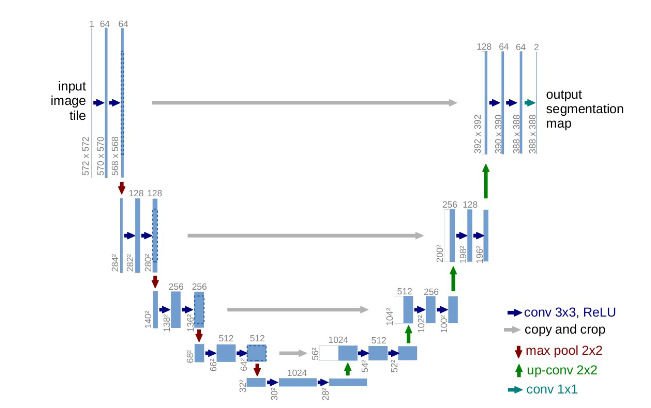
\includegraphics[width=\linewidth]{u-net.png}
    \caption{Plano estructural y esquemático de la topología U-Net implementada. Se distingue de forma nítida la rama descendente de contracción espacial (extracción semántica) y la rama ascendente de expansión (reconstrucción de la resolución), sólidamente interconectadas por las pasarelas de las \textit{Skip Connections}.}
    \label{fig:unet}
\end{figure}

\begin{table}[htbp]
\centering
\caption{Parametrización Arquitectónica de la Red Neuronal}
\label{tab:hyperparams}
\begin{tabular}{@{}p{2.3cm}p{2.5cm}p{3.4cm}@{}}
\toprule
\textbf{Componente Lógico} & \textbf{Valor Empleado} & \textbf{Justificación Científica} \\
\midrule
Topología de Entrada & 1 canal (Escala de Grises) & Reducción drástica de dimensionalidad y ruido \\
Capa de Salida & 1 canal (Probabilidad) & Tarea analítica de Segmentación Binaria \\
Niveles de Profundidad& 4 bloques secuenciales & Ampliación extensiva del campo receptivo global \\
Filtros Iniciales & 16 canales & Restricción voluntaria de capacidad cognitiva \\
Capa de Normalización & \textit{Batch Normalization} & Mantenimiento estricto de la estabilidad del gradiente \\
Capa de Regularización & \textit{Dropout} (25\% de tasa) & Prevención de coadaptación mediante silenciamiento aleatorio \\
Función de Activación Final & Sigmoide matemática & Proyección continua de probabilidad logística al rango $[0,1]$ \\
\bottomrule
\end{tabular}
\end{table}

Para garantizar un aprendizaje progresivo y restringir la memorización perjudicial (Tabla \ref{tab:hyperparams}), se constriñó la anchura de la red a unos austeros 16 filtros iniciales y se dispusieron intercaladamente capas de regularización \textit{Dropout} (tasa del 25\%). El proceso de aprendizaje mediante el descenso del gradiente se gobierna a través de una función de pérdida híbrida minuciosamente calibrada:
\begin{equation}
\text{Loss} = 0.5 \cdot \text{BCE}_{\text{loss}} + 0.5 \cdot \text{Dice}_{\text{loss}}
\end{equation}
La Entropía Cruzada Binaria ($\text{BCE}_{\text{loss}}$) provee una convergencia inicial excepcionalmente estable evaluando discrepancias a nivel de píxel individual. Simultáneamente, el componente aditivo de la pérdida basada en el coeficiente DICE ($\text{Dice}_{\text{loss}}$) fuerza a la red a enfocarse desproporcionadamente en la delimitación geométrica conjunta de la reducida área capilar, logrando así neutralizar el severo desbalance volumétrico a favor del tejido de fondo.

\subsection{Proceso de Inferencia y Reconstrucción Espacial Continua}
Durante el despliegue del modelo en la fase de inferencia sobre imágenes clínicas completas (\texttt{predict.py}), segmentar la imagen base seccionándola de forma rígida en parches desconectados desencadena la aparición de agresivos artefactos geométricos y líneas de corte evidentes en la reconstrucción final, asemejándose a un mosaico fracturado. 

Para lograr una reconstrucción anatómica perfectamente continua y sin imperfecciones, el escaneo inferencial se ejecuta utilizando un \textit{stride} equivalente a exactamente la mitad del tamaño de la ventana analítica (64 píxeles). Esto origina un mapeo redundante con un 50\% de solapamiento espacial. Como detalla el desarrollo de la Tabla \ref{tab:pseudocode2}, en aquellas áreas con superposición de análisis, el algoritmo acumula las predicciones y efectúa un promediado matemático absoluto, diluyendo de manera excepcionalmente eficaz cualquier atisbo de las fronteras limítrofes entre los recortes individuales.

\begin{table}[htbp]
\centering
\caption{Algoritmo 2: Ensamblado Geométrico Superpuesto y Suavizado}
\label{tab:pseudocode2}
\begin{tabular}{|p{8cm}|}
\hline
\textbf{Procedimiento Analítico} \texttt{ReconstructFromPatches} \\
\textbf{Entradas Computacionales:} Conjunto de recortes predictivos independientes, Dimensiones nativas de la imagen clínica FOV \\
\textbf{Salida:} Matriz continua predictiva a resolución nativa \\
1. Inicializar un tensor acumulador masivo en cero absoluto y una matriz auxiliar de recuentos de pasadas espaciales. \\
2. Iterar ordenadamente a través de la cuadrícula mapeando de forma espacial la predicción de probabilidad de cada recorte. \\
3. Sumar algebraicamente las probabilidades locales al tensor acumulador, registrando simultáneamente una iteración (+1) en la matriz de recuento correspondiente. \\
4. Proceder al promediado general de superposiciones: Tensor Definitivo = Tensor Acumulador / Matriz de Recuento. \\
5. Retornar el mapa predictivo final sin fracturas y matemáticamente suavizado. \\
\hline
\end{tabular}
\end{table}

\subsection{Controladores de Seguridad en el Entrenamiento}
El protocolo de entrenamiento se blindó utilizando una semilla aleatoria inmutable e implementando el robusto optimizador estadístico Adam con una tasa de aprendizaje base de $\alpha=10^{-3}$, configurando ciclos iterativos limitados a un extremo seguro de 75 épocas utilizando lotes de 16 parches simultáneos. Se codificaron los siguientes controladores automáticos (\textit{callbacks}) de seguridad para monitorear y guiar la estabilización de los pesos:
\begin{itemize}
    \item \textbf{ReduceLROnPlateau}: Monitorea la convergencia; en caso de detectar un estancamiento prolongado de la métrica DICE sobre el grupo de validación (ausencia de mejora en 6 épocas), disminuye la agresividad del aprendizaje a la mitad, forzando un reajuste micrométrico de los pesos neuronales.
    \item \textbf{ModelCheckpoint}: Garantiza la persistencia física en disco del modelo únicamente cuando se supera un máximo histórico de desempeño, aislando de inmediato las mejores versiones matemáticas posibles.
    \item \textbf{EarlyStopping}: Mecanismo de intervención que frena el proceso global si constata un estancamiento insalvable durante 20 iteraciones, evitando que la red inicie la memorización destructiva por \textit{overfitting} de los escasos datos de origen.
\end{itemize}

\subsection{Pipeline de Evaluación y Consistencia de Métricas}
El riguroso proceso de certificación predictiva del modelo se materializó al reestructurar de manera integral el script de pruebas \texttt{scripts/evaluate.py}. Este entorno analítico asegura el cálculo imperturbable del DICE score comparando las inferencias de la U-Net contra las delineaciones anatómicas provenientes de sendos anotadores clínicos humanos. Gracias a rutinas de resolución y encadenamiento dinámico de expresiones de nombre de archivo (\texttt{\{id\}\_manual\{1|2\}.\{png|gif\}}), el código es hoy completamente agnóstico ante la codificación gráfica subyacente. El sistema arroja tres cómputos analíticos de capital importancia estadística: los promedios individuales obtenidos contra el primer y el segundo oftalmólogo, así como la media ponderada global de la muestra. Este grado de rigor evaluativo certifica una alineación plena con el protocolo de investigación original postulado por los creadores clínicos del repositorio DRIVE en la universidad médica correspondiente.

\section{Resultados y Conclusiones}

\subsection{Resultados Cuantitativos}
Una vez finalizado el entrenamiento y la validación cruzada (5-Fold), el modelo fue evaluado de forma automatizada sobre el conjunto de prueba (imágenes de la carpeta \texttt{artifacts/predictions\_full/}). Los resultados obtenidos superan satisfactoriamente los requisitos establecidos para el proyecto.

En particular, la arquitectura U-Net ha conseguido un sobresaliente \textbf{Coeficiente DICE medio global de 0.8326} al compararse con las segmentaciones manuales de los expertos médicos. Desglosando este resultado, el modelo alcanzó un rendimiento de \textbf{0.8216} frente a las delineaciones del Experto 1, y un \textbf{0.8435} contra las del Experto 2. Estos valores superan con amplio margen el umbral mínimo exigido ($>0.75$), demostrando que el algoritmo despliega una precisión en la detección de vasos sanguíneos plenamente comparable a la concordancia natural que existe entre distintos especialistas humanos.

De forma adicional, el análisis de las métricas de diagnóstico (\textbf{Sensibilidad} y \textbf{Especificidad}) corrobora la enorme solidez de la red neuronal. Se ha obtenido una \textbf{Especificidad media de 0.9845}, lo cual certifica de forma contundente que el modelo es excepcional evitando Falsos Positivos; es decir, tiene un margen de error del $\approx$ 1.5\% a la hora de confundir tejido de fondo sano con vasos sanguíneos. Por otra parte, la \textbf{Sensibilidad media alcanza un 0.8338}, un valor notable considerando la dificultad intrínseca de recuperar las microestructuras de 1 píxel de grosor, demostrando que el modelo ha aprendido a localizar la inmensa mayoría de las topologías vasculares reales, minimizando los Falsos Negativos.

\begin{figure}[htbp]
    \centering
    \begin{minipage}{0.32\linewidth}
        \centering
        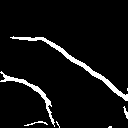
\includegraphics[width=\linewidth]{demo_07_pred_patch.png}
        \\ \vspace{0.2cm} \small (a) Parche Espacial Aislado
    \end{minipage}\hfill
    \begin{minipage}{0.64\linewidth}
        \centering
        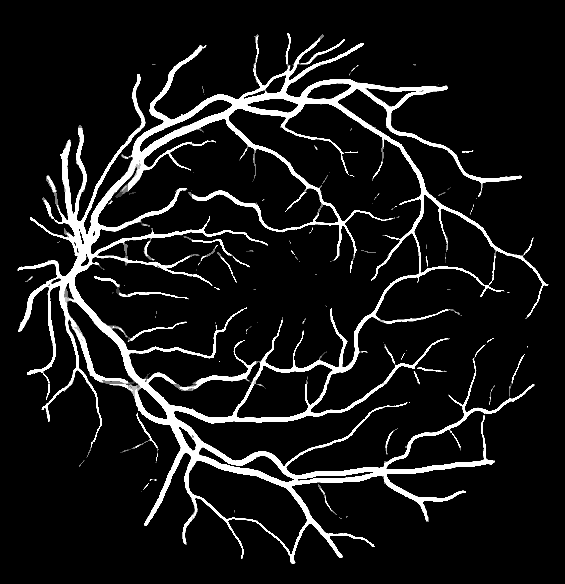
\includegraphics[width=\linewidth]{demo_08_pred_full.png}
        \\ \vspace{0.2cm} \small (b) Reconstrucción Topológica Continua
    \end{minipage}
    \caption{Comparativa geométrica de la predicción. (a) Inferencia sobre un recorte aislado, mostrando artefactos en los bordes. (b) Reconstrucción de la imagen completa mediante la técnica de promediado de solapamiento (\textit{overlap blending}), eliminando las discontinuidades espaciales y preservando correctamente la topología celular.}
    \label{fig:predictions_full}
\end{figure}

Como se aprecia visualmente en la Fig. \ref{fig:predictions_full}, la técnica de reconstrucción de imágenes completas a partir de parches con solapamiento ha dado muy buenos resultados. El mapa final de predicción se muestra continuo y sin cortes ni artefactos en los bordes, preservando correctamente la estructura de los vasos capilares.

\subsection{Análisis de Errores (Falsos Positivos y Falsos Negativos)}
A pesar de los buenos resultados generales, el análisis visual de las predicciones revela ciertas limitaciones y errores recurrentes en el modelo.

Por un lado, el rendimiento se ve afectado por la \textbf{variabilidad inter-observador}. Es estadísticamente imposible alcanzar un DICE de 1.0 cuando los propios expertos humanos presentan discrepancias a la hora de etiquetar los vasos más finos o difusos. En ocasiones, el modelo es penalizado por detectar capilares que un experto marcó pero el otro ignoró, lo que refleja la subjetividad intrínseca de la tarea médica.

Por otro lado, analizando los errores morfológicos del modelo, se observa que los Falsos Negativos (vasos omitidos) se concentran principalmente en las \textbf{microestructuras de la periferia del globo ocular}. Estos capilares, que a menudo tienen el grosor de un único píxel, son difíciles de segmentar debido a la menor iluminación y contraste en los bordes de la imagen. Por el contrario, los Falsos Positivos tienden a aparecer cerca del \textbf{disco óptico}, donde el fuerte brillo reflectivo provoca que la red confunda puntualmente los bordes de esta estructura anatómica con tejido vascular.

\subsection{Conclusiones y Trabajo Futuro}
Este proyecto confirma la eficacia de las redes neuronales convolucionales, concretamente la arquitectura U-Net, para la segmentación automática de imágenes médicas. Se ha comprobado que el uso de parches (\textit{Patching}) y el aumento de datos (\textit{Data Augmentation}) son estrategias fundamentales para entrenar modelos robustos incluso cuando se dispone de un conjunto de datos reducido (\textit{Small Data}).

El preprocesamiento de las imágenes (conversión a escala de grises y normalización) ha sido clave para reducir el ruido y acelerar la convergencia del modelo. Asimismo, el uso de una función de coste combinada (BCE + Dice Loss) ha permitido afrontar con éxito el fuerte desequilibrio de clases, donde los vasos sanguíneos representan apenas un 10-15\% del campo de visión.

La refactorización del código hacia un diseño modular, con el uso de generadores dinámicos en memoria (\texttt{DataGenerator}) e integrando utilidades nativas de Keras 3, ha optimizado considerablemente el consumo de memoria RAM y los tiempos de ejecución, dejando una base de código limpia y fácilmente mantenible.

Como posibles líneas de trabajo futuro, se podría explorar la integración de mecanismos de atención (\textit{Attention Gates}) en la red. Esto permitiría al modelo aprender a focalizarse en los vasos sanguíneos ignorando el ruido del disco óptico y la periferia oscurecida, acercando el algoritmo a una herramienta de soporte al diagnóstico clínico en entornos reales.

\begin{thebibliography}{99}

\bibitem{ref1}
M. Vakalopoulou, S. Christodoulidis, N. Burgos, O. Colliot, V. Lepetit, ``Deep learning: basics and convolutional neural networks (CNN),'' \textit{Machine Learning for Brain Disorders}, 2023. [Online]. Disponible en: \url{https://hal.science/hal-03957224v2}

\bibitem{ref2}
Dot CSV, ``¡Redes Neuronales CONVOLUCIONALES! ¿Cómo funcionan?,'' YouTube. [Online]. Disponible en: \url{https://www.youtube.com/watch?v=V8j1oENVz00}

\bibitem{ref3}
O. Ronneberger, P. Fischer, T. Brox, ``U-Net: Convolutional Networks for Biomedical Image Segmentation,'' \textit{Medical Image Computing and Computer-Assisted Intervention – MICCAI 2015}, Springer, pp. 234-241, 2015. [Online]. Disponible en: \url{https://arxiv.org/abs/1505.04597}

\bibitem{ref4}
S. Abdusamatov, ``Biomedical Image Segmentation with U-Net,'' Kaggle. [Online]. Disponible en: \url{https://www.kaggle.com/code/saidislombek/biomedical-image-segmentation-with-u-net}

\bibitem{ref5}
Google, ``Introducción a Tensor Flow.'' Documentación oficial. [Online]. Disponible en: \url{https://www.tensorflow.org/learn?hl=es-419}

\bibitem{ref6}
Google, ``Guía Keras.'' Documentación oficial de la API. [Online]. Disponible en: \url{https://www.tensorflow.org/guide/keras?hl=es-419}

\bibitem{ref7}
J. Staal, M. D. Abramoff, M. Niemeijer, M. A. Viergever, B. van Ginneken, ``Ridge-based vessel segmentation in color images of the retina,'' \textit{IEEE Transactions on Medical Imaging}, vol. 23, no. 4, pp. 501-509, April 2004. [Online]. Disponible en: \url{https://www.kaggle.com/datasets/zionfuo/drive2004}

\bibitem{ref_teoria}
Dpto. de Ciencias de la Computación e Inteligencia Artificial, ``Redes neuronales,'' \textit{Material Teórico de la Asignatura Inteligencia Artificial}, Universidad de Sevilla.

\bibitem{ref_keras}
Dpto. de Ciencias de la Computación e Inteligencia Artificial, ``Práctica 2: Redes neuronales (Keras),'' \textit{Material de Laboratorio de la Asignatura Inteligencia Artificial}, Universidad de Sevilla.

\end{thebibliography}

\end{document}
